\renewcommand{\thepage}{S\arabic{page}}  
\renewcommand{\thesection}{S\arabic{section}}   
\renewcommand{\thetable}{S\arabic{table}}   
\renewcommand{\thefigure}{S\arabic{figure}}
\setcounter{figure}{0}

% \section{Metropolis Evaluation}
% \counterwithin{figure}{section} %reset figure numbering

% The Hastings/Gibbs algorithm was evaluated for 450,000 iterations, with the first 10,000 discarded as burn-in iterations, during which the sampling algorithm was experiencing transient behavior. Such a large number of iterations allows for convergence of all parameter distribution. Our method is based on a markov chain, such that the proposed parameter values for each iteration depend on the values from the last accepted iteration according to:
% \begin{equation}\label{eqn:proposal}
% \begin{split}
% \Delta&=Range(prior) \\
% Proposal_i&=Accepted_{i-1} + \delta p \cdot (0.5-rand) \cdot \Delta; 
% \end{split}\tag{S1}
% \end{equation}
% where $\Delta$ is the range allowed by the uniform prior for each parameter and $rand$ is a random number between 0 and 1. $Proposal_i$ is the value of a parameter for iteration $i$ and $Accepted_{i-1}$ is the previous value of that parameter accepted by the algorithm. To more efficiently explore parameter space, proposed parameters were selected with step sizes $\delta p_{Age}$ = 0.1 and $\delta p_{TWTT}$ = 0.1 for those parameters associated with each likelihood in Equation~\ref{eqn:bigproblem}.

% The evaluation of the two likelihood functions (i.e. ``cost") are independently accepted according to each function's metropolis probability during each iteration. The accepted solutions for each cost, depth, and age are shown in Figure~\ref{fig:cost}. As seen in the figure, these cost values show sufficient mizing to suggest posterior distributions are stationary.

% \begin{figure*}[ht]
% %\begin{center}
% \centering
% 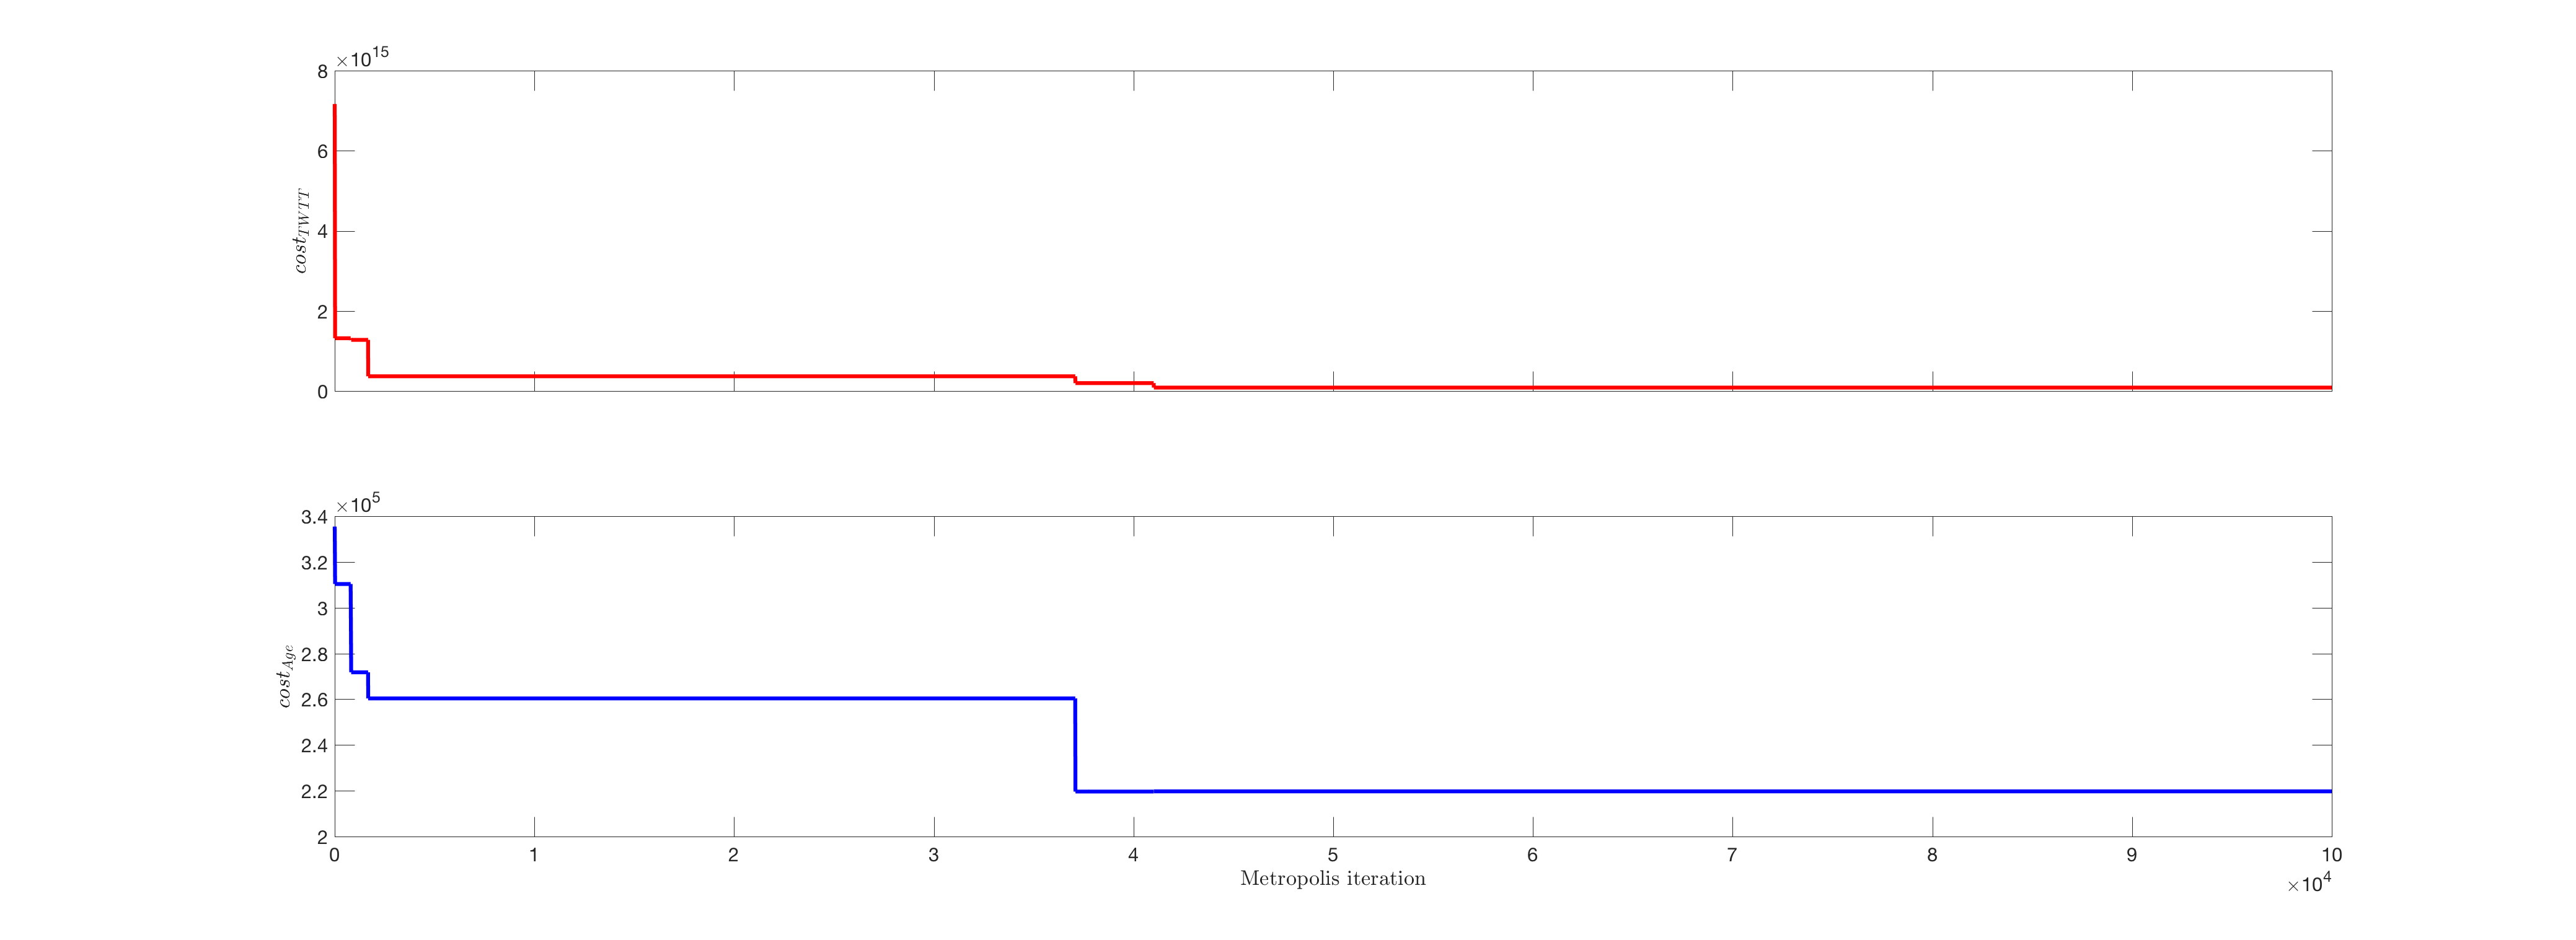
\includegraphics[scale=0.4]{../analysis/figures/cost}
% %\captionsetup{width=.9\textwidth}
% \caption[]{Cost of the age and depth likelihood functions at each accepted iteration for the Byrd ice core site.}
% %\end{center}
% \label{fig:cost}
% \end{figure*}





% \section{Regularization}\label{sec:regularization}
% \counterwithin{figure}{section} %reset figure numbering

% Sampling accumulation rate parameters along the depth profile is inefficient and problematic because many proposed solutions are unrealistically variable. We expect the mean accumulation rate over time (and therefore depth) changes slowly and continuously. To improve our accumulation rate solutions, we regularize the likelihood of reflector age. A regularization parameter is added to the age cost term which punishes proposed accumulation rate profiles which are highly variable relative to a solution computed with no regularization and smoothed over a moving 600-m depth window. This window size is chosen because it is the smallest interval over which the data can be smoothed given the 200-m bin size of the accumulation rate parameters. 

% The regularization term, $r$ is the ratio of the variance of a proposed set of accumulation rates to the variance of the smoothed, non-regularized accumulation rate profile. Values of the regularization term for accepted parameter solutions are shown in Figure~\ref{fig:reg}. The regularization is weighted as $r^6$ when included in the calculation of the age cost (Equation~\ref{eqn:loglikeage}) to sufficiently reduce variability in the accumulation rate profile. 


% \begin{figure*}[ht]
% %\begin{center}
% \centering
% 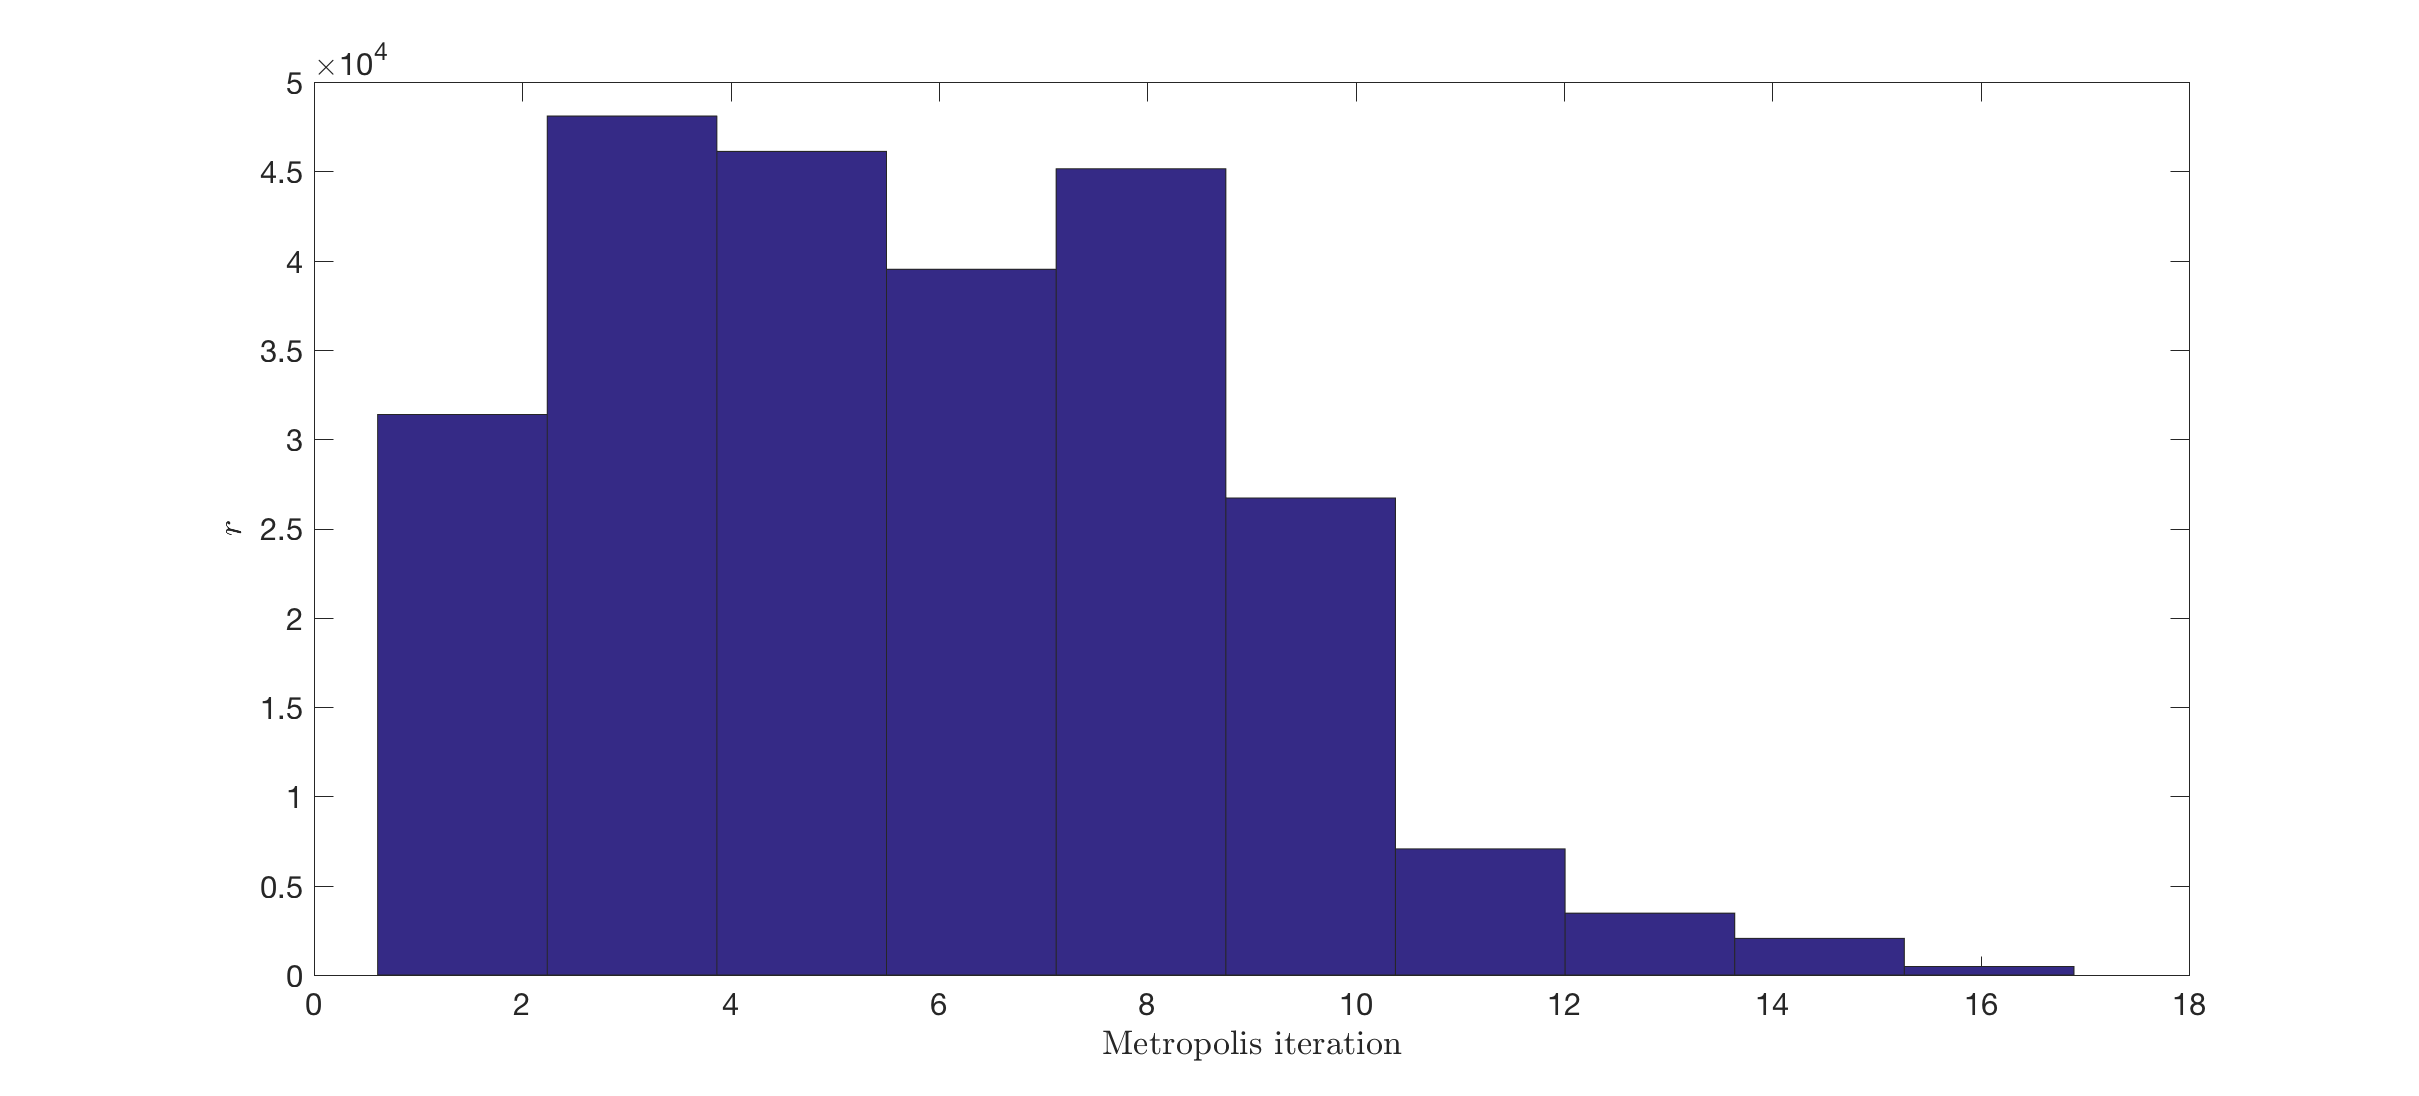
\includegraphics[scale=0.4]{../analysis/figures/regularization}
% %\captionsetup{width=.9\textwidth}
% \caption[]{Values of the regularization parameter at each accepted metropolis iteration.}
% %\end{center}
% \label{fig:reg}
% \end{figure*}








% \section{Estimating TWTT uncertainty}\label{sec:sigmatwtt}
% \counterwithin{figure}{section} %reset figure numbering
% To estimate $\sigma_{TWTT}$ in Equation~\ref{eqn:loglikeage}, we assume a perfect model then perturb it with errors consistent what we expect to find in the data. We assume the depth errors can be described by a gaussian distribution which results in the following relationship between the cost, degrees of freedom, and $\sigma_{TWTT}$ \citep{jackson&huerta2016}.


% \begin{equation}
% \frac{1}{\sigma_{TWTT}}= \frac{\sqrt{k_e/2}}{\sigma_{{E_m}^*}}\tag{S2}
% \end{equation}
% Here $k_e$ is the effective number of degrees of freedom and ${E_m}^*$ represents the perfect model of TWTT which is perturbed with errors consistent with what we expect to find in the radar observations. For simplicity, we assume $k_e$ is the same as the number of reflectors for which we invert.

% This method makes use of the ``perfect model":
% \begin{equation}
% cost^*_{TWTT} = \frac{\sum_{j = z}[TWTT_m(z) - \overline{TWTT_m}(z)]^2}{2}
% \end{equation}


% \section{Byrd ice core volcanic chronology}\label{sec:volcanic}

% Table of those points from the 50ka record used (i.e. ones with unique depths at 1-m model resolution)





% \section{Parameter correlation}\label{sec:ke}
% %\counterwithin{figure}{section} %reset figure numbering



% Figure~\ref{fig:flowparamconvergence} shows the results of inverting for several model parameters in this problem, including flow parameters such as $q$ as well as ice property parameters such as $v_{ice}$. The results show the parameters are not correlated with one another and do seem to convergence to most-likely solutions.

% \begin{figure*}[ht]
% %\begin{center}
% \centering
% \makebox[\textwidth][c]{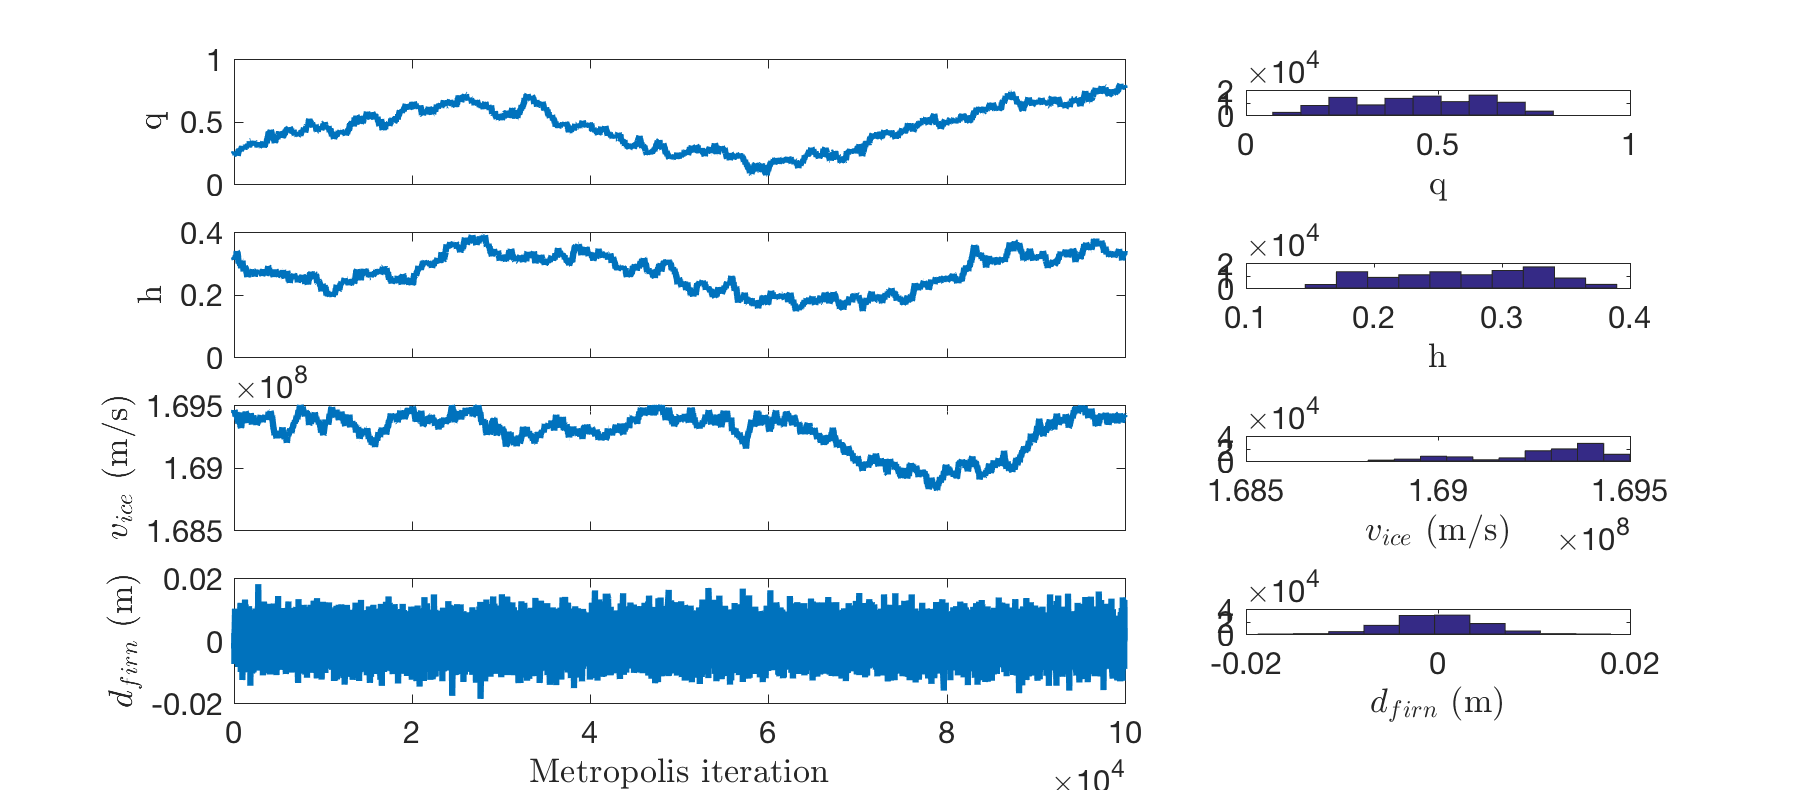
\includegraphics[scale=0.4]{../analysis/figures/convergence1}}
% %\captionsetup{width=.9\textwidth}
% \caption[]{Left: Flow parameter values at each accepted Metropolis iteration for parameters $q$ (top), $h$, $v_{ice}$, and $d_{firn}$ (bottom). The parameter values do not appear correlated. Right: Histograms of the parameter values shown in the left column. Histograms show the parameter values converging.}
% %\end{center}
% \label{fig:flowparamconvergence}
% \end{figure*}

% Accumulation rate is divided into 10 parameters, each covering a depth bin of $\sim$200 m. This allows for variation in the accumulation rate over time, as expected. The resulting accumulation rate profiles are shown in Figure~\ref{fig:accumdepth}. As discussed elsewhere in the Supplemental Information, these profiles have been regularized to preferentially select those which do not exhibit unrealistic variability. In Figure~\ref{fig:accumdepth}, they have been additionally sorted by cost to demonstrate the relative quality of the accepted solutions.

% \begin{figure*}[ht]
% %\begin{center}
% \centering
% \makebox[\textwidth][c]{\includegraphics[scale=0.4]{../analysis/figures/accumdepthSorted}}
% %\captionsetup{width=.9\textwidth}
% \caption[]{Accumulation rate as a function of ice depth colored by cost value for the estimated parameter values. (Accumulation rate series associated with lower cost are expected to be solutions.) Accumulation rate is estimated in 10 depth bins at $\sim$200 m depth intervals. Transitions between these intervals have been smoothed in this figure for each of viewing.}
% %\end{center}
% \label{fig:accumdepth}
% \end{figure*}

% To further explore the accumulation rate solutions, we look at the accepted parameter values and their convergence over all iterations. As seen in the right side of Figure~\ref{fig:accumconvergence}, the accumulation rate solutions do not converge as readily as other parameters, leaving wider distributions exhibiting more uncertainty in our estimates of accumulation rate. This may mean that our priors play an important role in estimating the value of accumulation rate and therefore the result could be improved with a more informative prior. This is particularly true at the bottom of the ice column, where neither volcanic chronology data nor radar data is available to constrain the accumulation rate.

% We see correlation between some accumulation rate parameters (left side of Figure~\ref{fig:accumconvergence}). This may indicate we could have combined these accumulation rate depth bins. Figure~\ref{fig:accumCorrelation} shows a correlation matrix between pairs of accumulation rate parameters. Along the diagonal are histograms of each accumulation rate parameter. Pairs of accumulation rate parameters to not tend to be very correlated and only one pair of accumulation rate parameters has $R^2 > 0.5$. In general, $R^2$ values are highest between accumulation rates in the lower part of the ice column, where parameter values are more difficult to constrain due to a lack of data and flatter age-depth profile.


% \begin{figure*}[ht]
% %\begin{center}
% \centering
% \makebox[\textwidth][c]{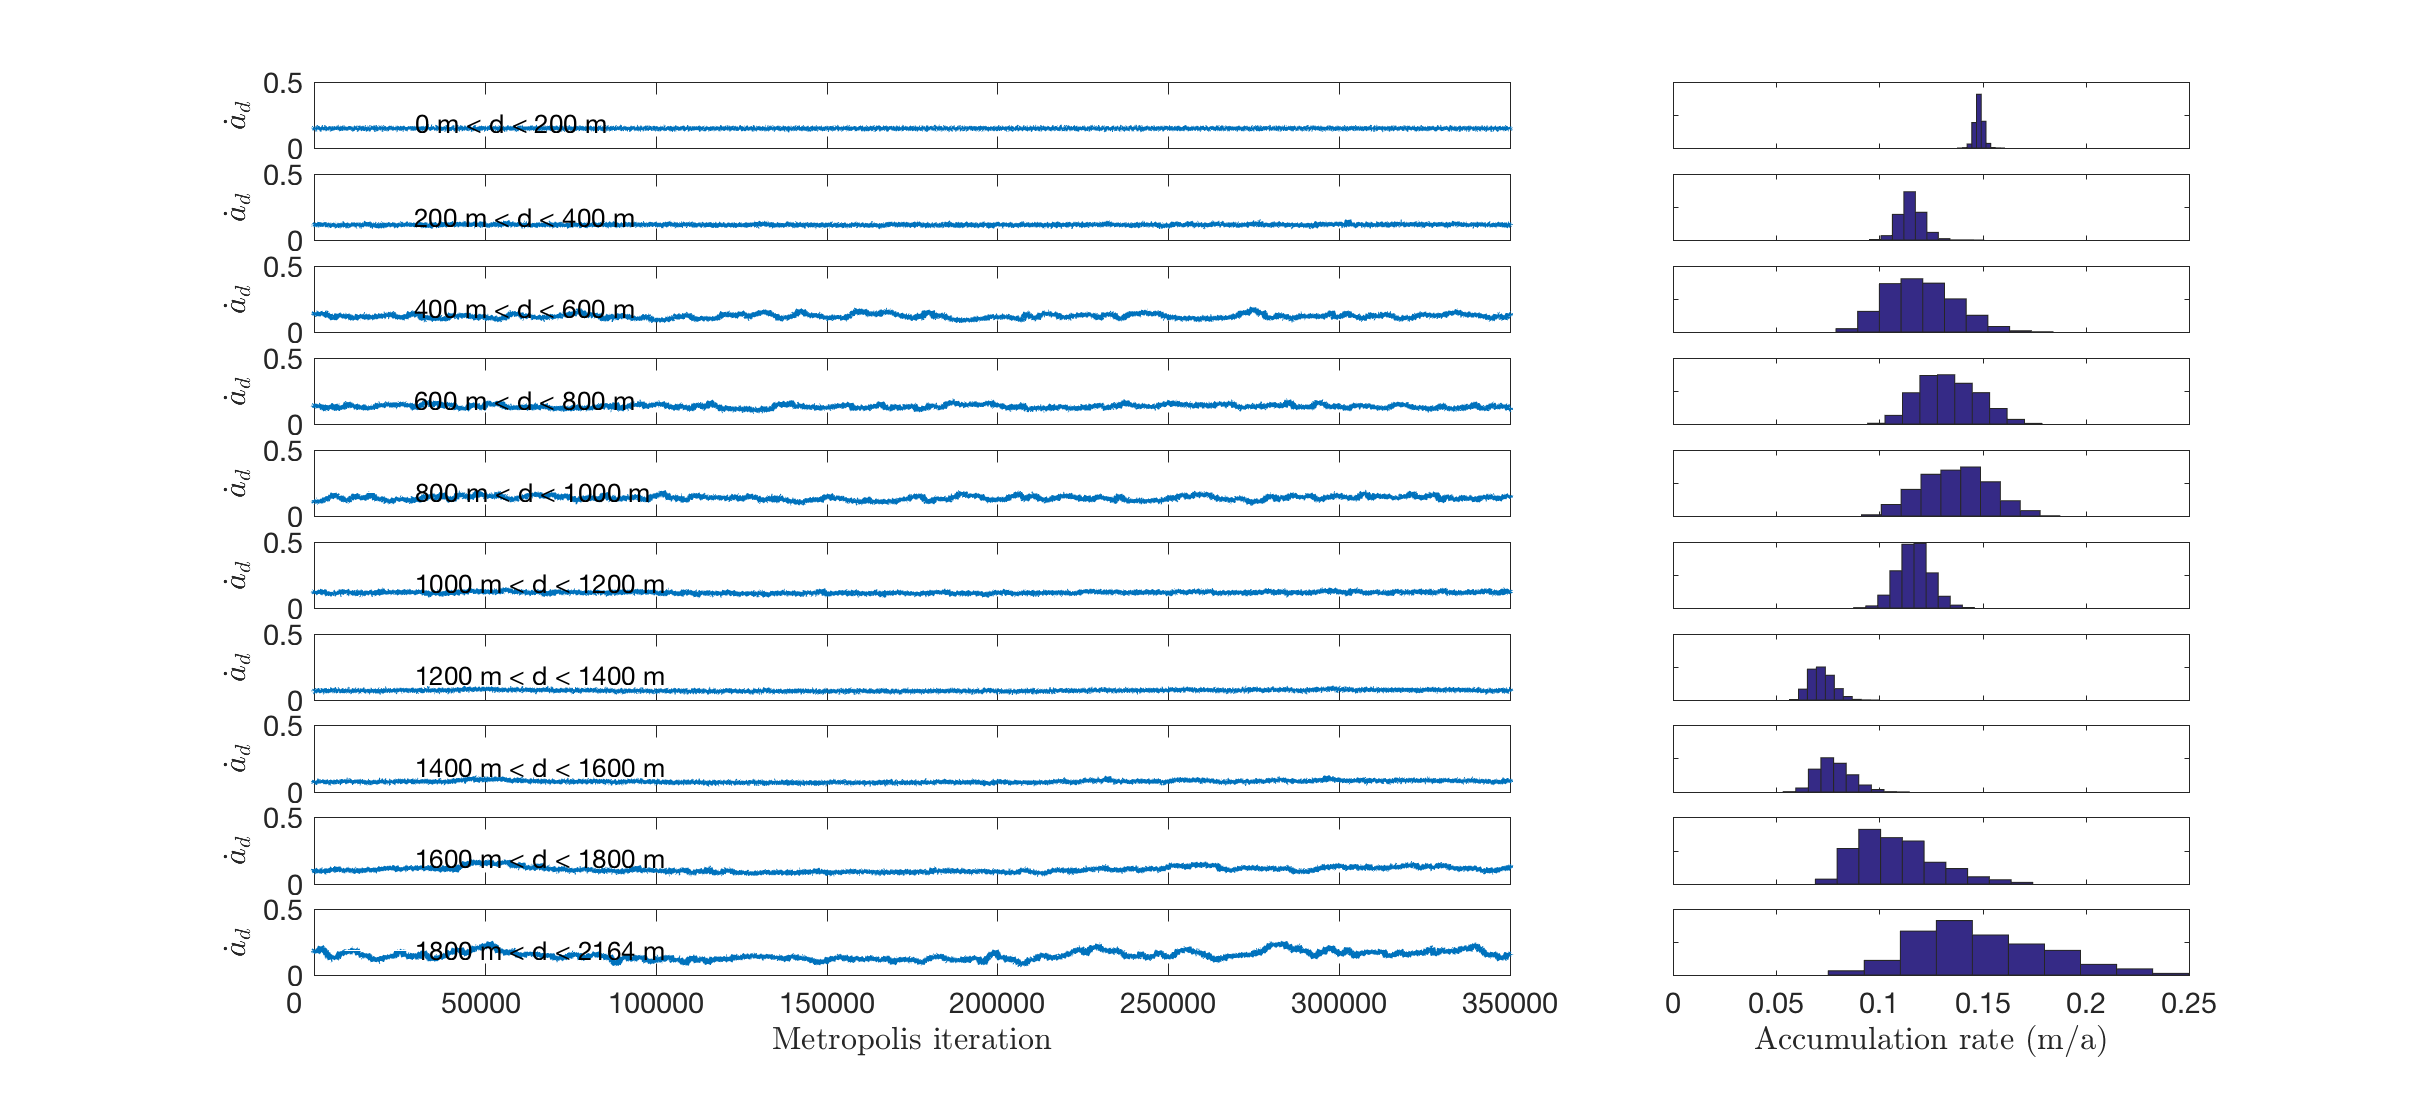
\includegraphics[scale=0.4]{../analysis/figures/convergence2}}
% %\captionsetup{width=.9\textwidth}
% \caption[]{Left: Values of each accumulate rate parameter (in each of 11 depth bins, shallowest at top). Right: Histograms of the parameter values at left. Certain depth bins appear to be correlated and the histograms of values are wider, indicating the accumulation rate parameters are slower to converge and more uncertain.}
% %\end{center}
% \label{fig:accumconvergence}
% \end{figure*}

% \begin{figure*}[ht]
% %\begin{center}
% \centering
% \makebox[\textwidth][c]{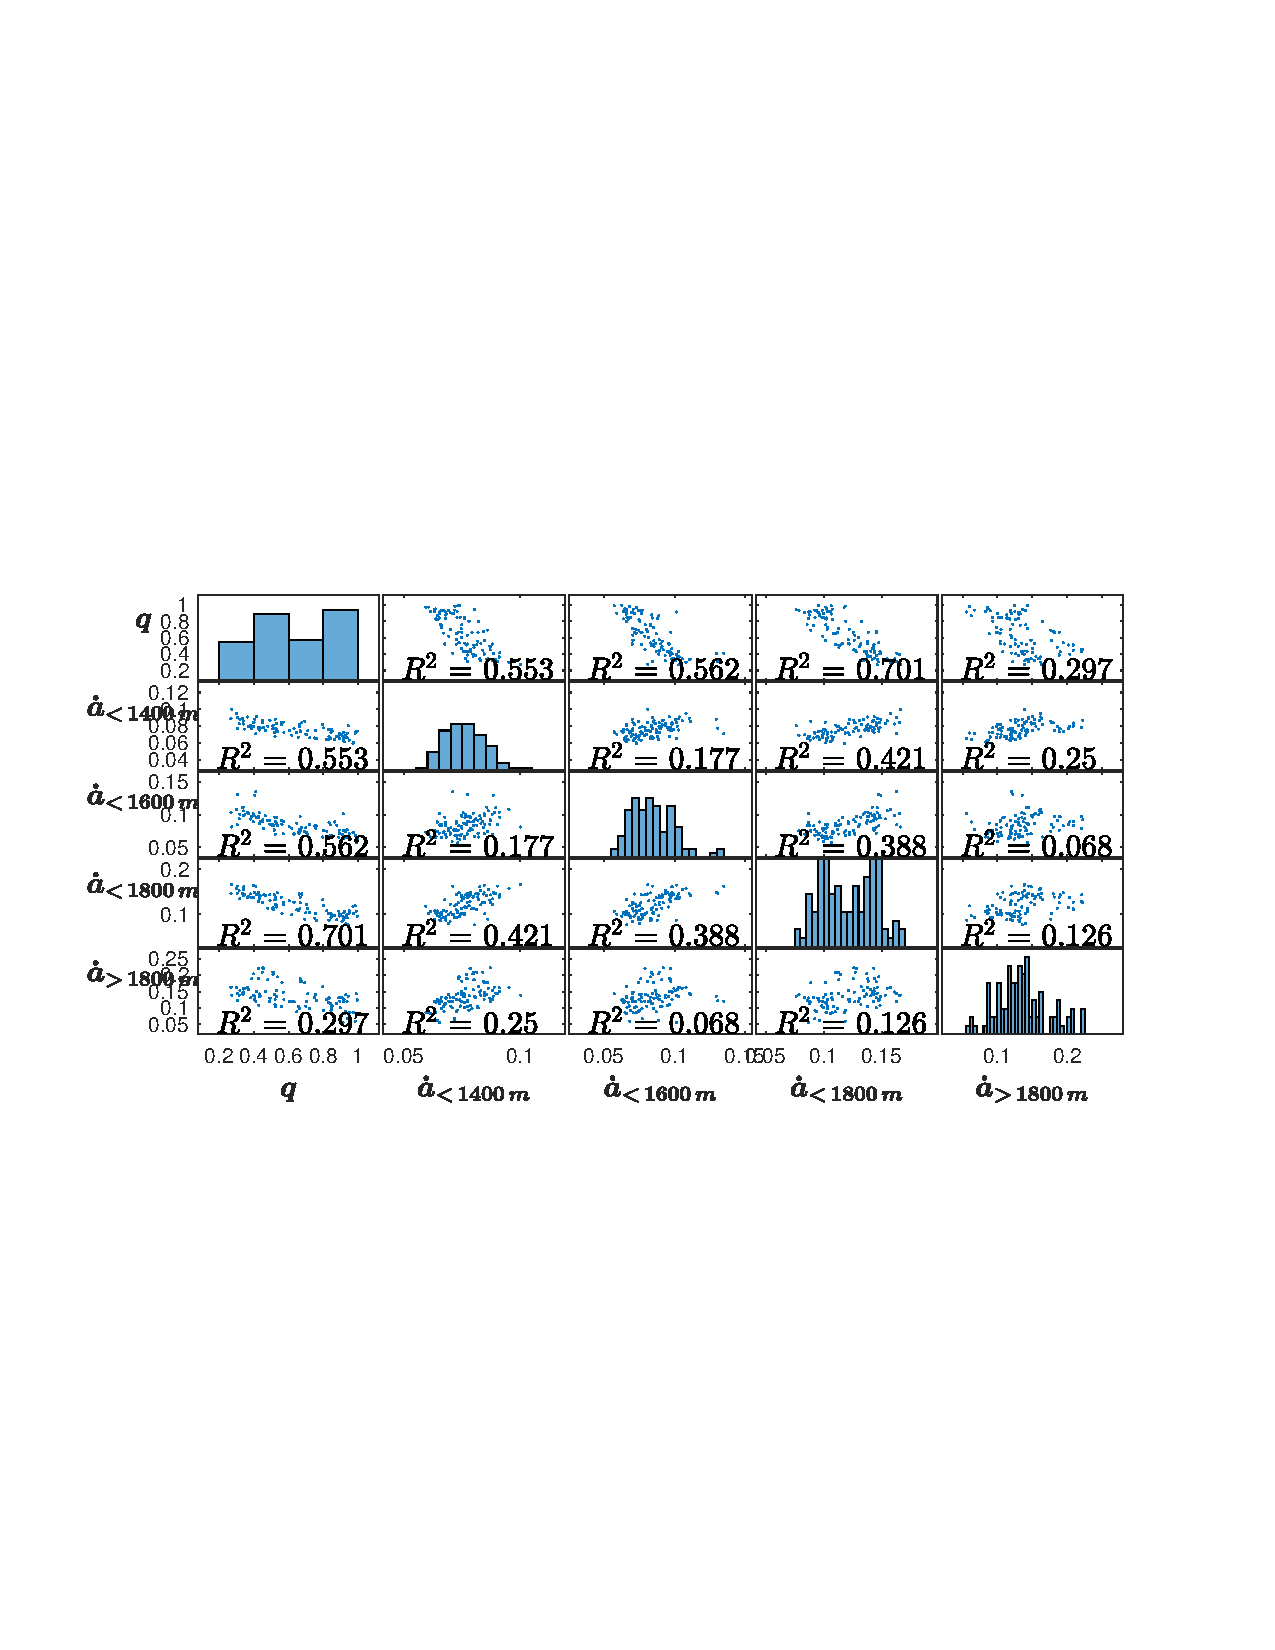
\includegraphics[scale=0.4]{../analysis/figures/accumCorrelation}}
% %\captionsetup{width=.9\textwidth}
% \caption[]{Correlation of each accumulation rate parameter with every other accumulation rate parameter. Histograms of each accumulation rate are shown along the diagonal. Pairs of parameters with $R^2 > 0.5$ have their correlation coefficients shown in red.}
% %\end{center}
% \label{fig:accumCorrelation}
% \end{figure*}


% Convergence of the reflector depths is shown in Figure~\ref{fig:depthconvergence}.


% \begin{figure*}[ht]
% %\begin{center}
% \centering
% \makebox[\textwidth][c]{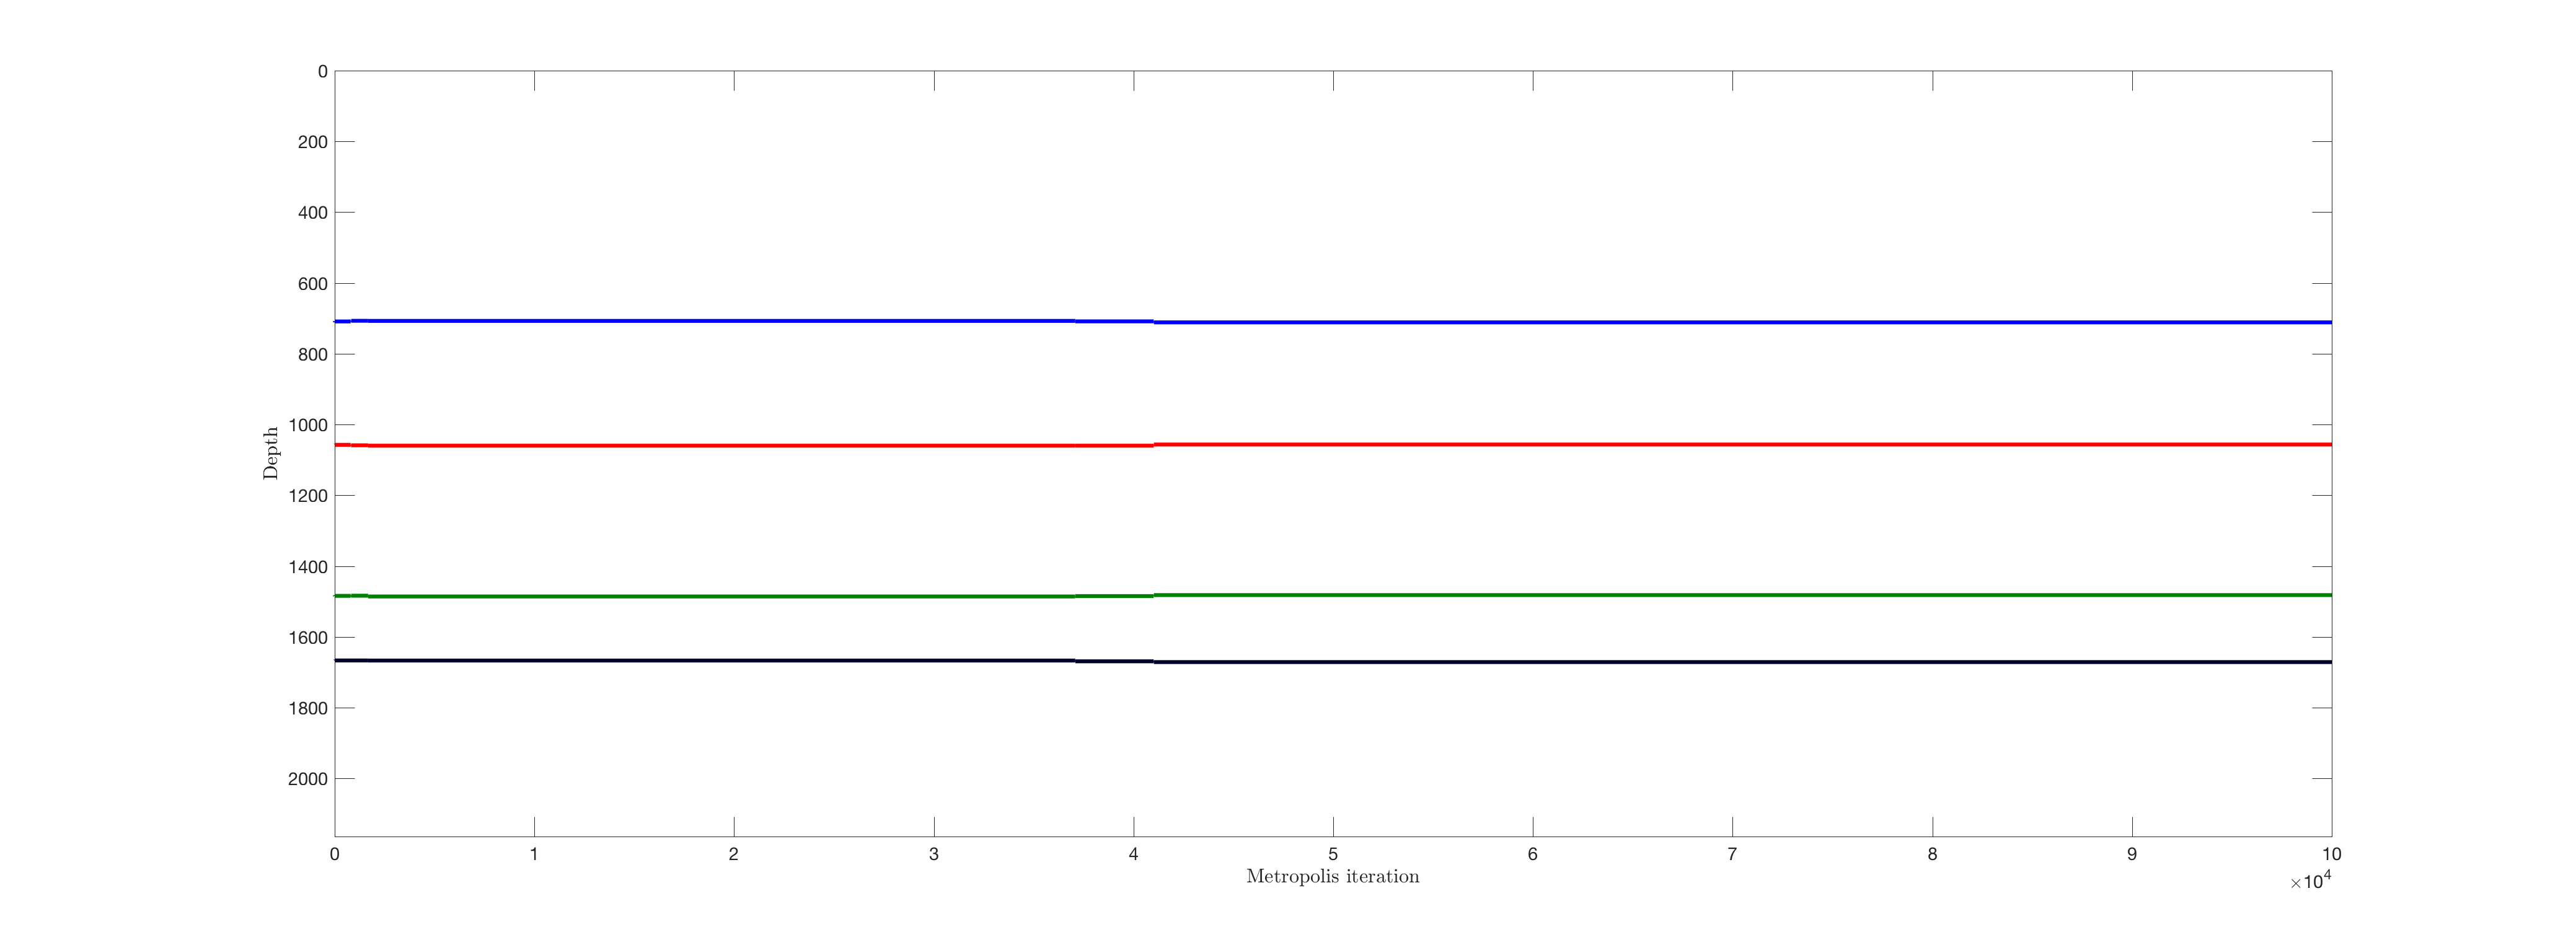
\includegraphics[scale=0.4]{../analysis/figures/convergence3}}
% %\captionsetup{width=.9\textwidth}
% \caption[]{Reflector depth values at each accepted metropolis iteration.}
% %\end{center}
% \label{fig:depthconvergence}
% \end{figure*}



% \section{Firn Correction}

% \begin{figure*}[h]
% %\begin{center}
% \centering
% 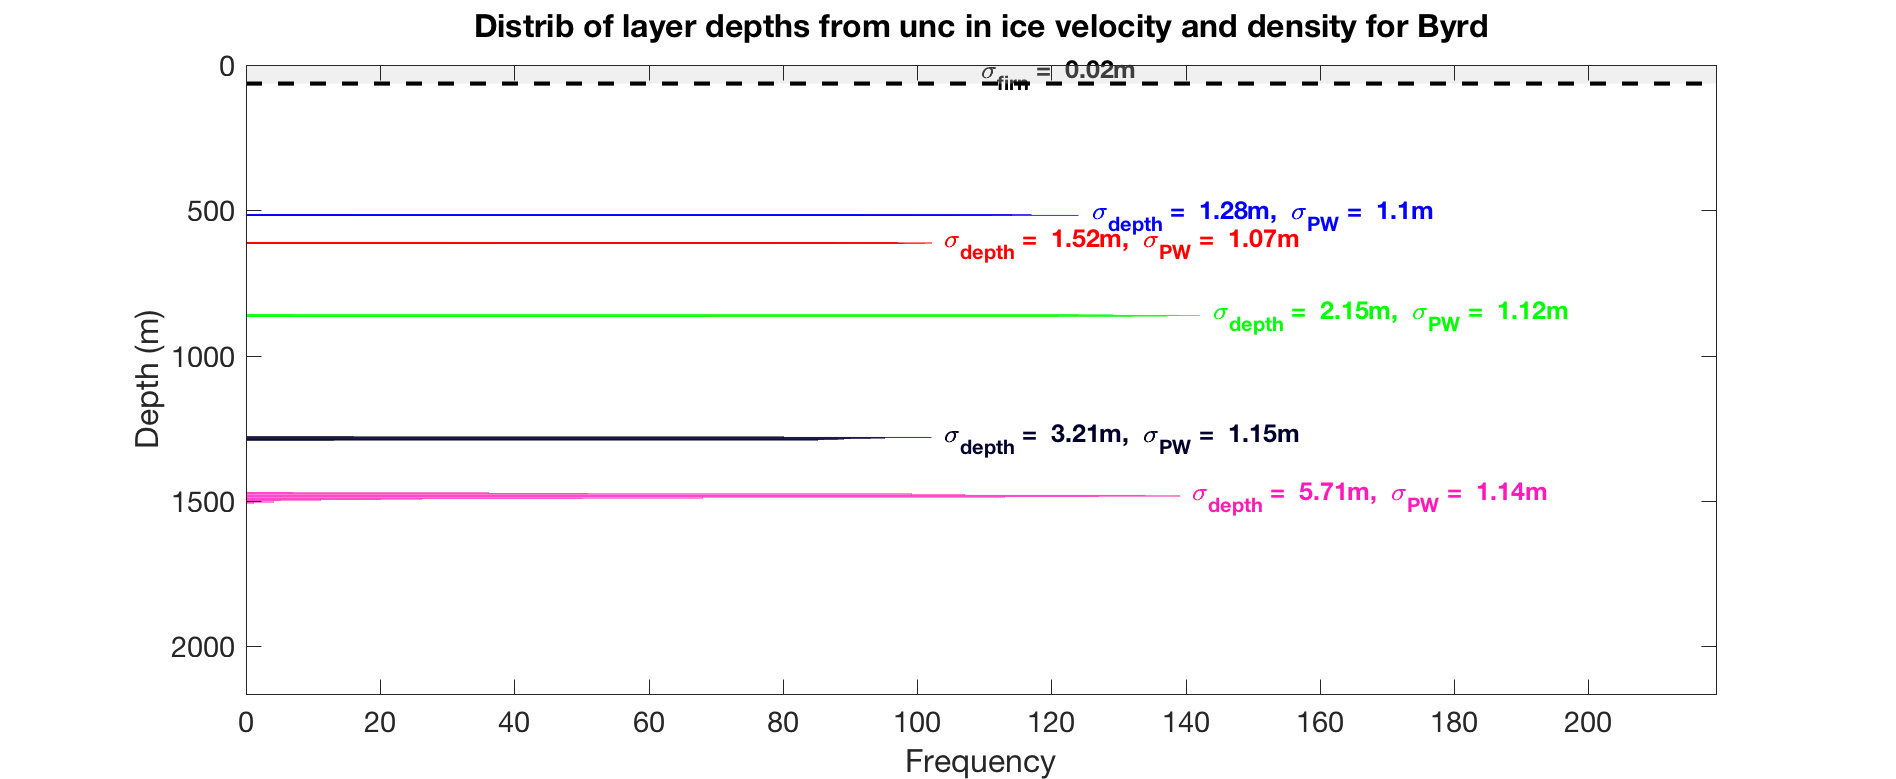
\includegraphics[scale=0.5]{figures/firncorrection}
% %\captionsetup{width=.9\textwidth}
% \caption[]{}
% %\end{center}
% \label{fig:firncorrection}
% \end{figure*}









